\documentclass{standalone}
\usepackage{tikz}
\begin{document}
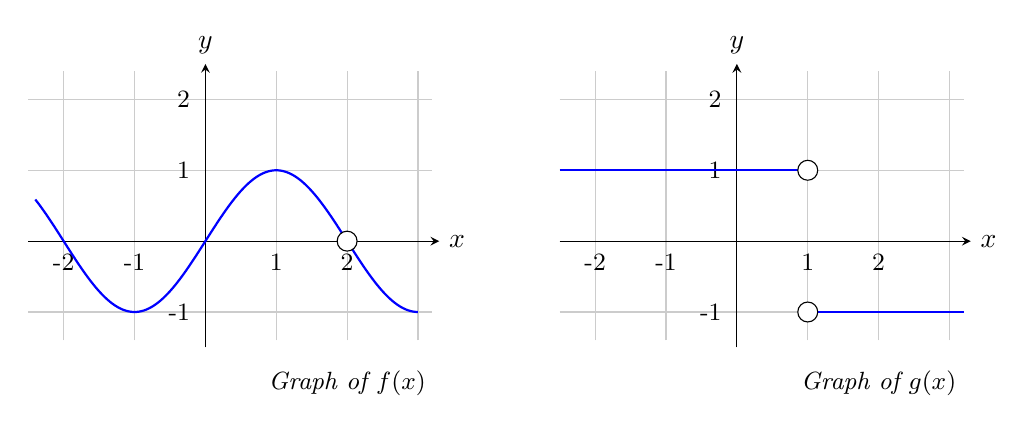
\begin{tikzpicture}[>=stealth, scale=0.9]
  % ---- Left graph: f(x) ----
  % Grid
  \draw[gray!40, thin] (-2.5,-1.4) grid (3.2,2.4);
  % Axes
  \draw[->] (-2.5,0) -- (3.3,0) node[right] {$x$};
  \draw[->] (0,-1.5) -- (0,2.5) node[above] {$y$};
  % x-axis ticks and labels
  \foreach \x in {-2,-1,1,2} {
    \node[below, font=\small] at (\x,-0.05) {\x};
  }
  % y-axis ticks and labels
  \foreach \y in {-1,1,2} {
    \node[left, font=\small] at (-0.08,\y) {\y};
  }
  % f(x) = sin(pi*x/2) on (-2.5, 2), open circle at (2, 0)
  \begin{scope}
    \clip (-2.5,-1.5) rectangle (3.2,2.5);
    \draw[blue, thick, domain=-2.4:3, samples=160]
      plot (\x, {sin(90*\x)});
  \end{scope}
  % Open circle at (2,0)
  \draw[fill=white, draw=black] (2,0) circle (4pt);
  % Label
  \node[font=\small\itshape] at (2.0,-2.0) {Graph of $f(x)$};

  % ---- Right graph: g(x) ----
  \begin{scope}[shift={(7.5,0)}]
    % Grid
    \draw[gray!40, thin] (-2.5,-1.4) grid (3.2,2.4);
    % Axes
    \draw[->] (-2.5,0) -- (3.3,0) node[right] {$x$};
    \draw[->] (0,-1.5) -- (0,2.5) node[above] {$y$};
    % x-axis ticks and labels
    \foreach \x in {-2,-1,1,2} {
      \node[below, font=\small] at (\x,-0.05) {\x};
    }
    % y-axis ticks and labels
    \foreach \y in {-1,1,2} {
      \node[left, font=\small] at (-0.08,\y) {\y};
    }
    % g(x) = 1 for x < 1, g(x) = -1 for x > 1
    \draw[blue, thick] (-2.5,1) -- (1,1);
    \draw[blue, thick] (1,-1) -- (3.2,-1);
    % Open circles at x=1 (both pieces)
    \draw[fill=white, draw=black] (1,1) circle (4pt);
    \draw[fill=white, draw=black] (1,-1) circle (4pt);
    % Label
    \node[font=\small\itshape] at (2.0,-2.0) {Graph of $g(x)$};
  \end{scope}
\end{tikzpicture}
\end{document}
